\documentclass[a4paper,12pt]{article}
%\usepackage{fullpage}
%\usepackage{pdfpages}

\usepackage{geometry}
 \geometry{
 a4paper,
 total={170mm,257mm},
 left=20mm,
 top=20mm,
 }

\usepackage{color}
\usepackage{amsmath,graphicx,makeidx}
\usepackage{lscape}
\usepackage{fancyhdr}
\addtolength{\headheight}{1.5cm} % make more space for the header
\pagestyle{fancyplain} % use fancy for all pages except chapter start
\lhead{
\includegraphics[height=1.7cm]{FOSSEE-logo}} % left logo
\rhead{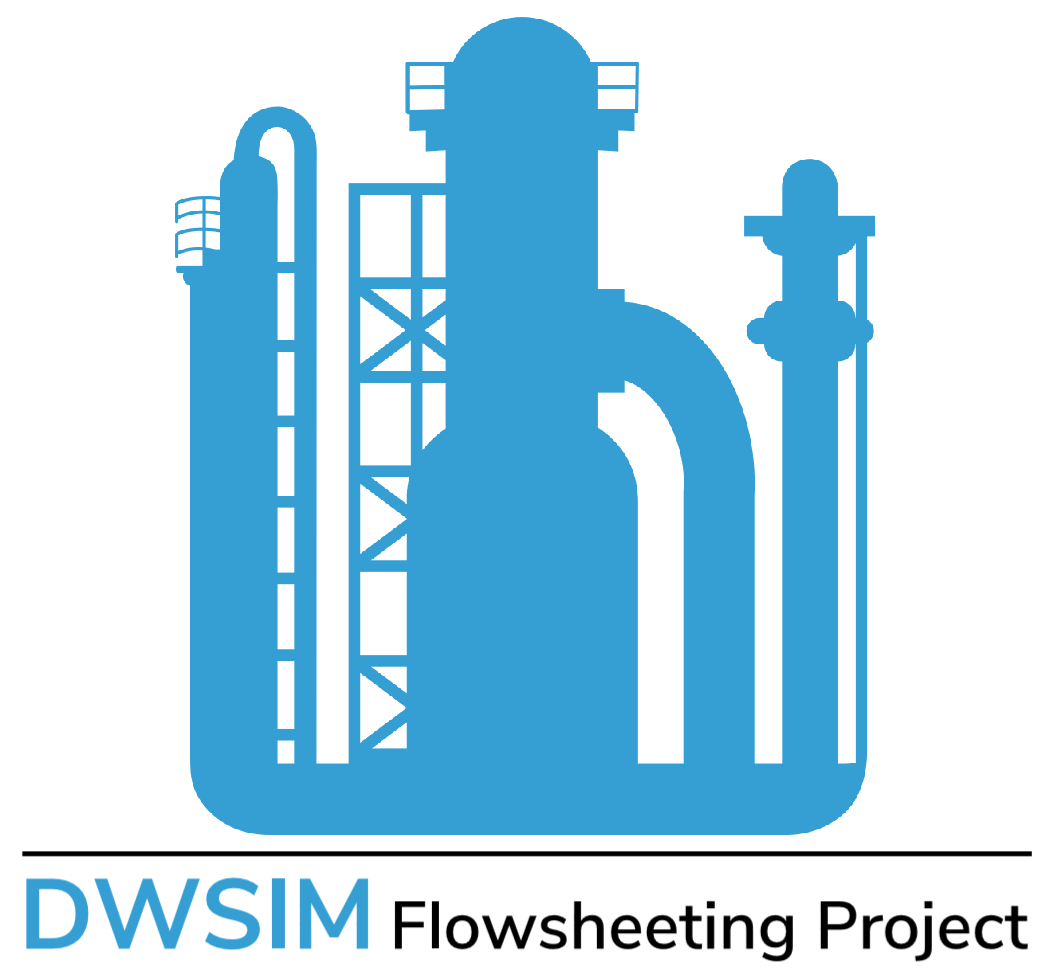
\includegraphics[height=3.5cm]{DWSIM-flowsheeting-project-logo}} % right logo
\renewcommand{\headrulewidth}{0pt} % remove rule below header

\title{Hydrogen Production through Methane Catalytic Steam Reforming}
\author{Daniel Wagner \\ DWSIM Developer}
\date{}

\begin{document}

\maketitle

\noindent \textbf{Background \& Description:}
\newline Natural gas has been proposed as a source of hydrogen for fuel cell vehicle applications because of the existing infrastructure. In a process known as steam reforming, natural gas and steam are reacted into mostly carbon monoxide and hydrogen with some carbon dioxide also produced. There can also be excess water in the reformate stream.

\bigskip A feed consisting of 10000 mol/h $CH_4$, 10000 mol/h $H_2O$, and 100 mol/h $H_2$ enters into a steam reforming reactor that operates at 1000 K and a 1 atm feed pressure. The reactions taking place in the PFR are as follows:

\noindent The steam reforming reaction is given as:

\begin{center} 
\noindent $CH_4 + H_2O \rightleftharpoons 3 H_2 + CO$ 
\end{center}				      

\noindent In the steam reformer, the water gas shift reaction also takes place as: 
\begin{center} 
\noindent $CO + H_2O \rightleftharpoons H_2 + CO_2$ 
\end{center}						           

\noindent Adding together the steam reforming and water gas shift reactions gives the overall reaction:  

\begin{center} 
\noindent $CH_4 + 2 H_2O \rightleftharpoons 4 H_2 + CO_2$ 
\end{center}

\bigskip In the reactor, methane ($CH_4$) and water ($H_2O$) are fed as reactants and carbon dioxide ($CO_2$), carbon monoxide ($CO$), and hydrogen ($H_2$) are produced over a nickel catalyst on an alumina support. The weight of the catalyst is 386 g. The reaction takes place in isothermal mode with reactor volume of 1 $m^3$. 75.62\% conversion is obtained for methane.

\vspace{5ex}
\centerline{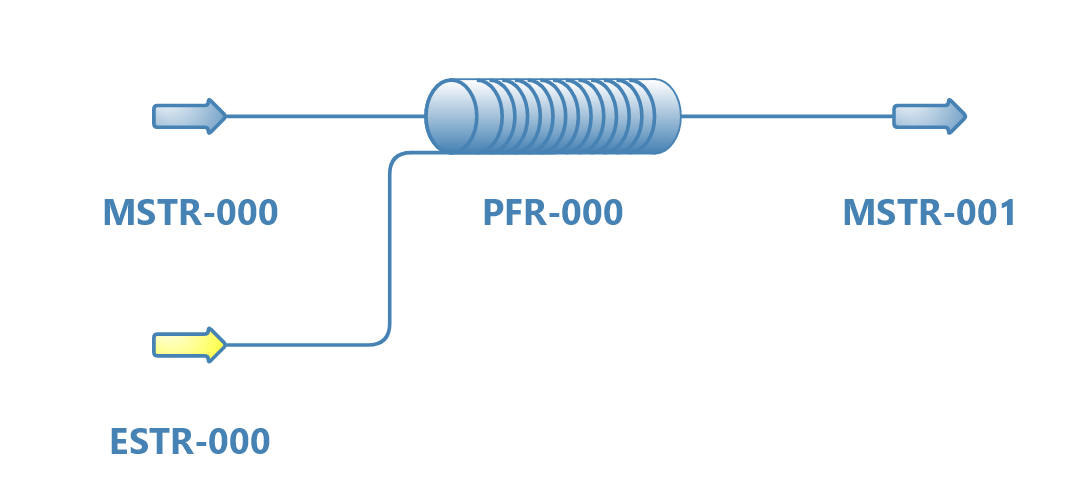
\includegraphics[width=1\linewidth]{H2-Prod.png}}
\centerline{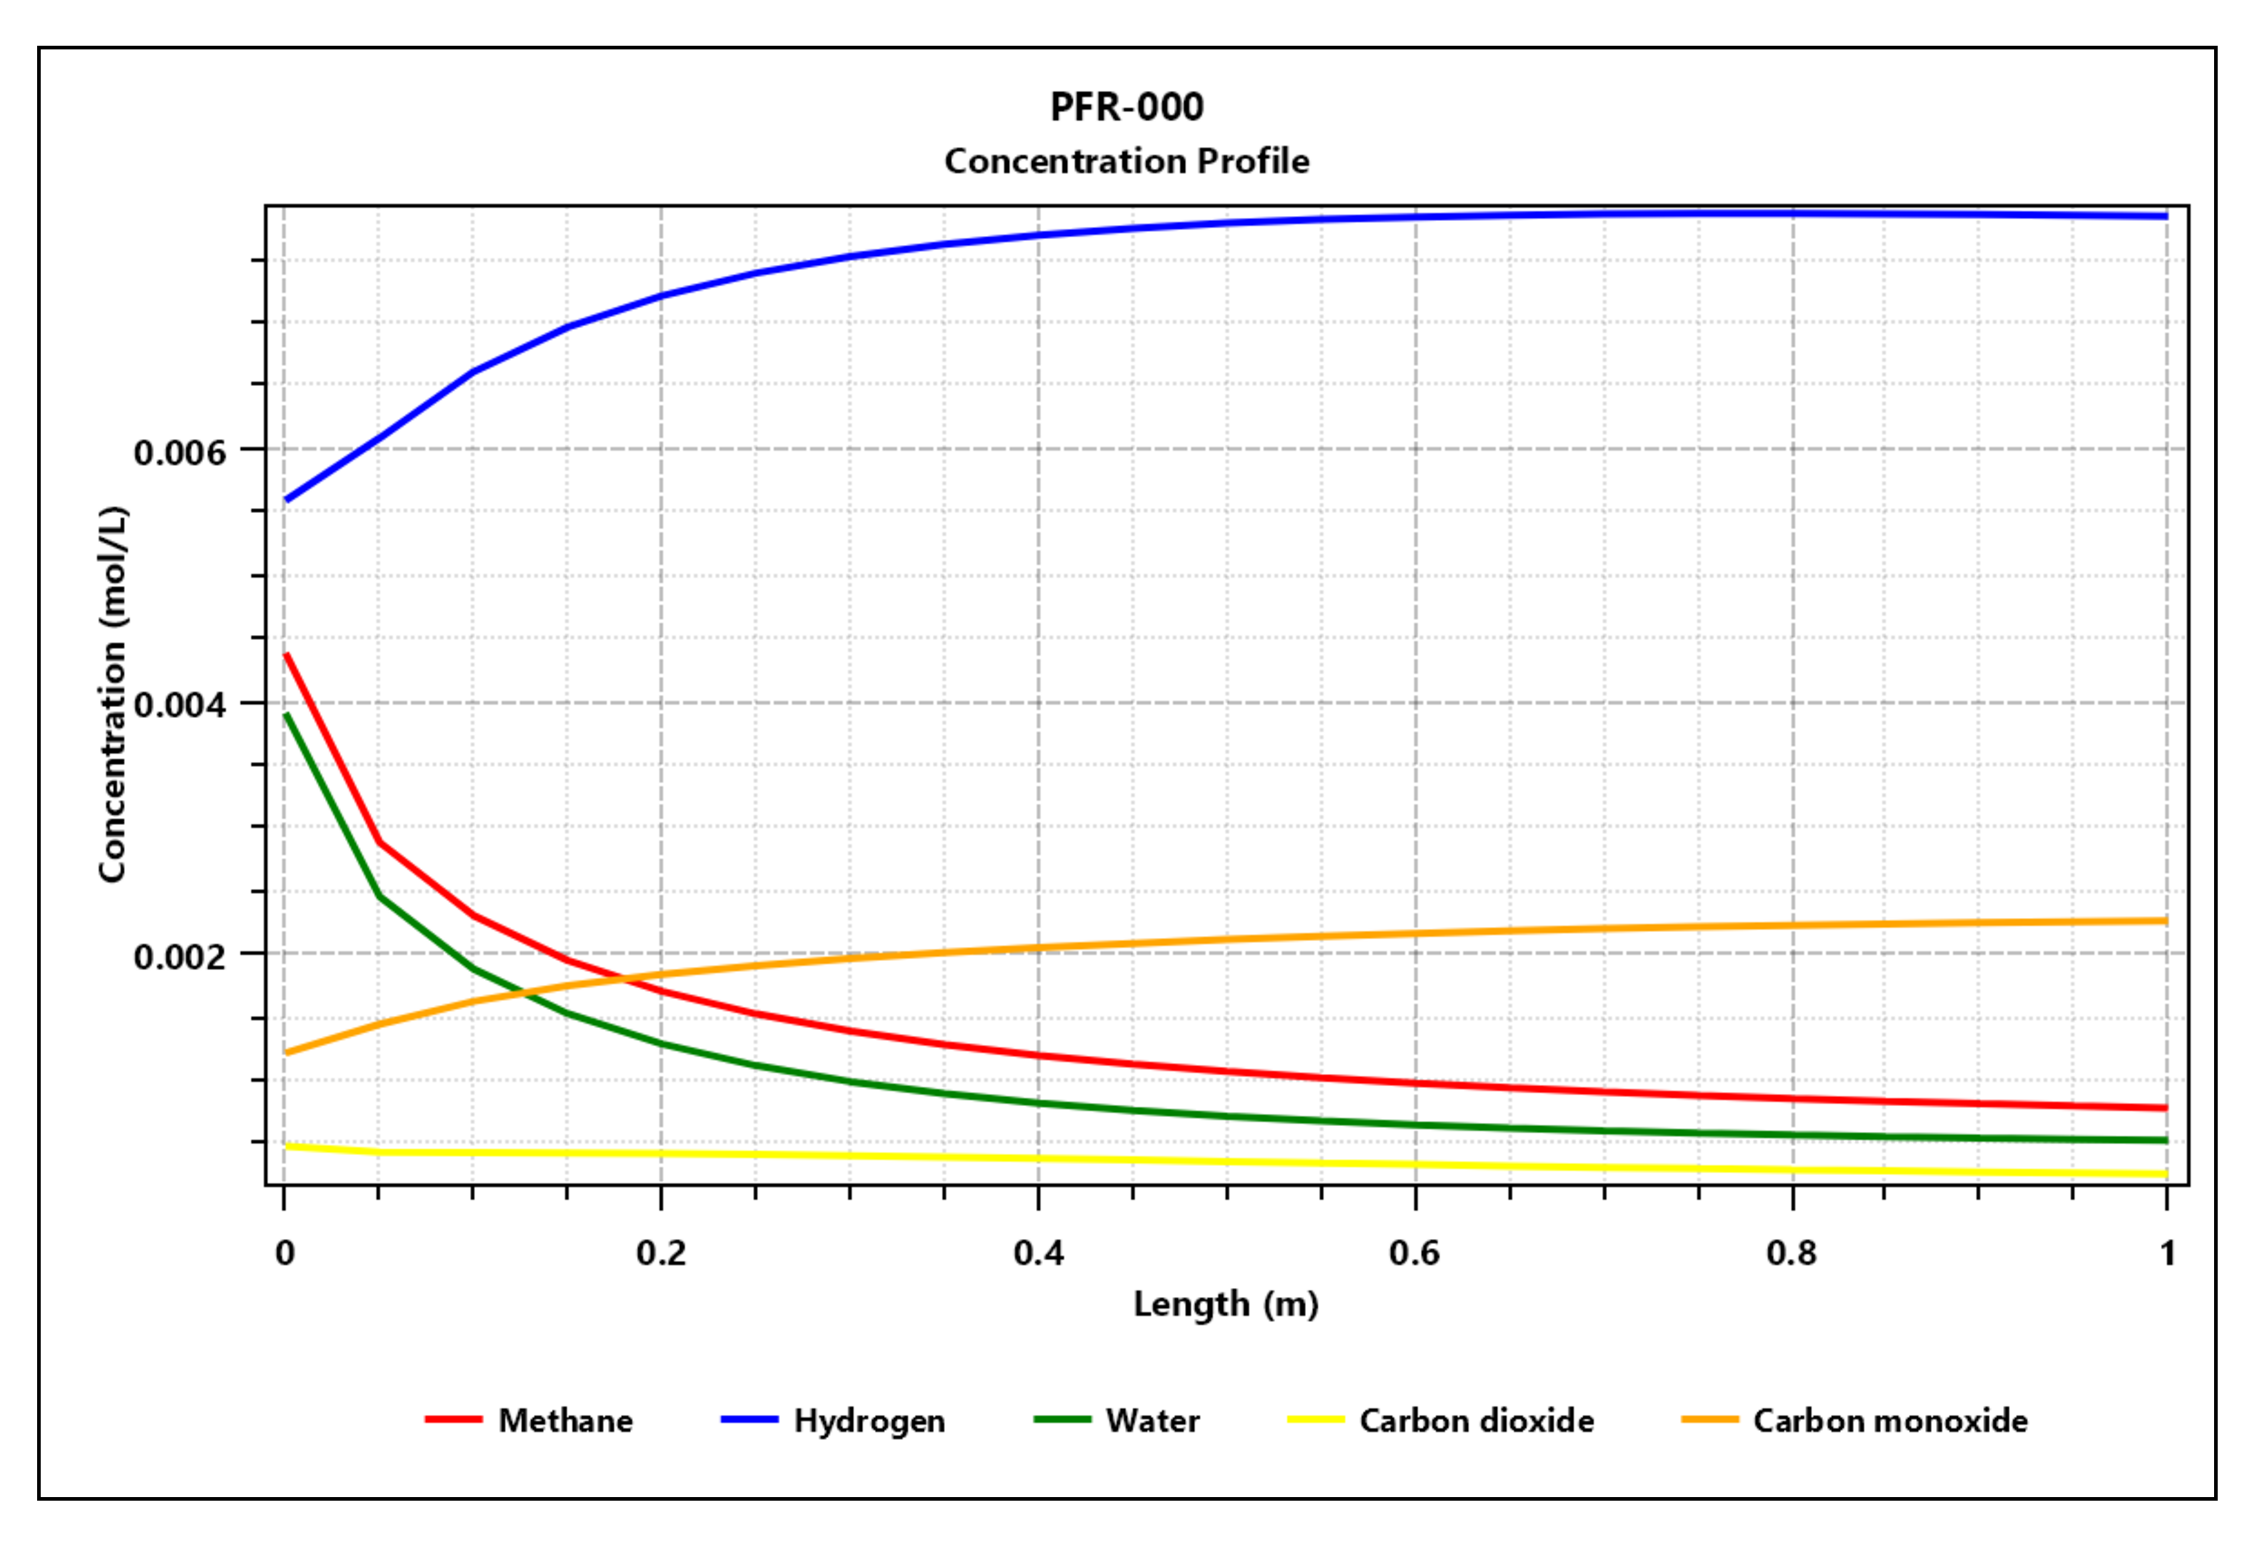
\includegraphics[width=0.8\linewidth]{Conc-Profile.png}}

\noindent \textbf{Results:}
\begin{table}[h]
\centering
%\resizebox{\textwidth}{!}{%
%\resizebox{\columnwidth}{!}{%
\scalebox{1.2}{%
\begin{tabular}{|l|l|l|l|}
\hline
\bf Object          & MSTR-001 & MSTR-000 &       \\ \hline
Temperature     & 726.85   & 726.85   & C     \\ \hline
Pressure        & 0.96143  & 1.01325  & bar   \\ \hline
Mass Flow       & 340.7791 & 340.7816 & kg/h  \\ \hline
Molar Flow      & 35381.14 & 20100    & mol/h \\ \hline
Volumetric Flow & 3060.166 & 1649.323 & m$^3$/h  \\ \hline
\end{tabular}%
}
\caption{Streamwise Results for Hydrogen Production thorugh Methane Catalytic Steam Reforming}
\end{table}

\end{document}


